\documentclass[10pt,a4paper]{article}
\usepackage[latin1]{inputenc}
\usepackage{amsmath}
\usepackage[scale=0.8]{geometry}
\usepackage{amsfonts}
\usepackage{outlines}
\usepackage{amssymb}
\usepackage{graphicx}
\begin{document}
	\begin{titlepage}
		\title{Important Facts to Consider in Modelling HBV MTCT\newline\newline\large{James Mba Azam\\SACEMA, Stellenbosch University}}
		\maketitle
	\end{titlepage}
	\begin{outline}
		\1 The decrease in MTCT
		of HBV would also decrease the reservoir of chronically
		infected individuals who could then transmit in early
		childhood or adulthood\cite{thio2015global}. 
		\1 Antiviral drugs given in the late first or early second
		trimester have the potential for decreasing maternal HBV
		DNA to undetectable concentrations at delivery \cite{thio2015global}.
		\1 Even when administered \textit{optimally}, the current
		immuno prophylaxis regimen fails in 8-32\% of mothers
		who have the highest risk of transmitting HBV - i.e,
		those who are HBeAg positive\cite{thio2015global}.
		\1 Although several factors have been associated with MTCT of HBV,
		studies have repeatedly shown that the most important
		risk factor is high circulating concentrations of HBV
		DNA in the mothers, with about 10$^7$ IU/mL being the
		cutoff\cite{thio2015global}.
		\1 Crucial research gaps include:
		\2  the timing and
		exact indication of the intervention,
		\2 establishment of a
		goal HBV DNA concentration to achieve at delivery,
		\2 determination of frequencies of maternal HBV flares
		after treatment discontinuation, and 
		\2 selection of the best antiviral drug
		\cite{thio2015global}.
		\1 Since human beings are the only reservoir of HBV,
		eradication is possible and an important step towards this
		goal is interruption of MTCT\cite{thio2015global}.
		\1 Hepatitis B immune globulin at the time of birth plus
		three doses of the recombinant hepatitis B vaccine over
		the first 6 months of life is up to 95\% effective in
		preventing perinatal transmission\cite{tran2009management}.
		\1 Antiviral treatment during the third trimester of pregnancy
		may reduce perinatal transmission of HBV; the benefit
		appears most pronounced with high maternal viremia\cite{tran2009management}.
		\1 Despite successful screening and vaccination programs,
	\textit{high maternal HBV DNA} correlates in some studies
		with perinatal transmission\cite{tran2009management}.
		\1 The disease-free equilibrium can be used as an indicator of possible eradication.
	\end{outline}
	\begin{figure}[p]
		\centering
		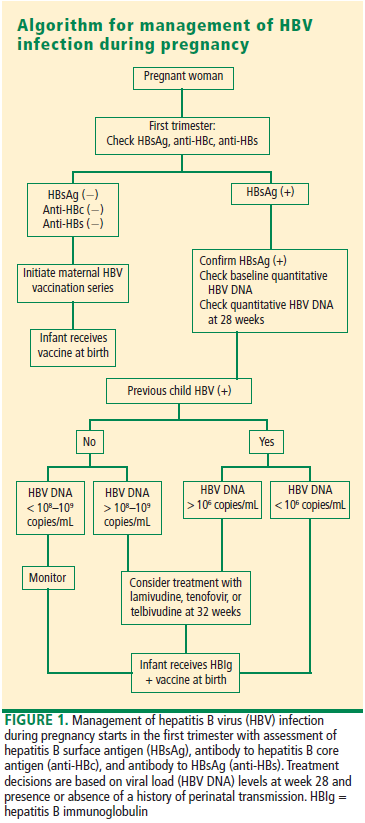
\includegraphics[width=13cm,height=25cm]{pic}
	\end{figure}
	\bibliographystyle{apalike}
	\bibliography{refs}
\end{document}